%%% Template originaly created by Karol Kozioł (mail@karol-koziol.net) and modified for ShareLaTeX use

\documentclass[11pt]{article}

\usepackage[T1]{fontenc}
\usepackage[utf8]{inputenc}
\usepackage{graphicx}
\usepackage{xcolor}
\usepackage{float}
\usepackage{tgtermes}
\usepackage{natbib}
%\usepackage[subnum]{cases}
\usepackage[super]{nth}
\bibpunct{(}{)}{;}{a}{}{,}
\usepackage{amsmath,amssymb}
\usepackage{enumerate}
\usepackage{multicol}
\usepackage{tikz}
\usepackage[amssymb]{SIunits}
\usepackage{rotating}
\usepackage{enumitem}
\usepackage{geometry}
\geometry{total={8.5in,11in},
left=1in,right=1in,%
bindingoffset=0mm, top=1in,bottom=1in}
\usepackage[super]{nth}
\usepackage[
pdftitle={Homework 1}, 
pdfauthor={Jeremy Gibbs, University of Utah},
colorlinks=true,linkcolor=blue,urlcolor=blue,citecolor=blue,bookmarks=true,
bookmarksopenlevel=2]{hyperref}

\linespread{1.1}
\setlength{\parskip}{1em}
\setlength{\parindent}{0pt}
\newcommand{\linia}{\rule{\linewidth}{0.5pt}}

\makeatletter
\renewcommand{\maketitle}{
\begin{center}
\vspace{2ex}
{\huge \textsc{\@title}}
\vspace{1ex}
\\
\linia\\
ME EN 7960-003 \hfill Homework \#3 Solutions \hfill Due: December \nth{1}
\vspace{4ex}
\end{center}
}
\makeatother
%%%

% custom footers and headers
\usepackage{fancyhdr,lastpage}
\pagestyle{fancy}
\lhead{}
\chead{}
\rhead{}
%\lfoot{Assignment \textnumero{} 5}
\cfoot{}
\rfoot{Page \thepage~/~\pageref*{LastPage}}
\renewcommand{\headrulewidth}{0pt}
\renewcommand{\footrulewidth}{0pt}
\usepackage{scalerel}[2014/03/10]
\usepackage{stackengine}
\usepackage{empheq}
\newcommand*\widefbox[1]{\fbox{\hspace{0.5em}#1\hspace{0.5em}}}

\newcommand\reallywidetilde[1]{\ThisStyle{%
  \setbox0=\hbox{$\SavedStyle#1$}%
  \stackengine{-.1\LMpt}{$\SavedStyle#1$}{%
    \stretchto{\scaleto{\SavedStyle\mkern.2mu\sim}{.5467\wd0}}{.4\ht0}%
%    .2mu is the kern imbalance when clipping white space
%    .5467++++ is \ht/[kerned \wd] aspect ratio for \sim glyph
  }{O}{c}{F}{T}{S}%
}}
\usepackage{cancel}
%

%%%----------%%%----------%%%----------%%%----------%%%

\begin{document}

\title{Large-Eddy Simulation of Turbulent Flows}

\maketitle

\begin{enumerate}

\item Using the basic properties of convolution filters and starting with the scalar conservation equation given by
\begin{displaymath}
\frac{\partial \theta}{\partial t} + u_i\frac{\partial \theta}{\partial x_i} = \frac{1}{ScRe}\frac{\partial^2 \theta}{\partial x_i^2}+Q :
\end{displaymath}

\begin{enumerate}
\item derive the filtered scalar conservation equation.  Clearly show each step in the process and clearly define the subfilter scale term.\\
\textcolor{blue}{We apply the filter
$$\reallywidetilde{\frac{\partial \theta}{\partial t}} + \reallywidetilde{u_i\frac{\partial \theta}{\partial x_i}} = \reallywidetilde{\frac{1}{ScRe}\frac{\partial^2 \theta}{\partial x_i^2}}+Q$$
Note that the filter commutes with differentiation and that:
$$\frac{\partial u_i \theta}{\partial x_i} = u_i\frac{\partial \theta}{\partial x_i} + \cancelto{0}{\theta\frac{\partial u_i}{\partial x_i}}\quad  \text{to arrive at}\quad
\frac{\partial \widetilde{\theta}}{\partial t} + \frac{\partial \widetilde{u_i \theta}}{\partial x_i} = \frac{1}{ScRe}\frac{\partial^2 \widetilde{\theta}}{\partial x_i^2}$$
We can decompose the unknown term following Leonard (1974) as
$$\widetilde{u_i \theta} = \widetilde{u_i}\widetilde{\theta} + q_i$$
where $q_i$ is the SFS scalar flux. The filtered scalar conservation equation is then given by
$$\boxed{\frac{\partial \widetilde{\theta}}{\partial t} + \frac{\partial \widetilde{u_i} \widetilde{\theta}}{\partial x_i} = \frac{1}{ScRe}\frac{\partial^2 \widetilde{\theta}}{\partial x_i^2} - \frac{\partial q_i}{\partial x_i}}$$
}
\item Use Leonard's decomposition (Leonard, Adv. Geophys. 1974) to decompose your answer to (a) and label terms that indicate the SFS Reynolds flux, interaction between resolved and unresolved scales, and the interaction amongst the smallest resolved scales (Leonard term).\\
\textcolor{blue}{Decompose the parts of the unknown term of $q_i$ by using $u_i = \widetilde{u}_i + u_i^\prime$ and $\theta = \widetilde{\theta} + \theta^\prime$
$$\widetilde{u_i \theta} = \reallywidetilde{(\widetilde{u}_i + u_i^\prime) (\widetilde{\theta} + \theta^\prime)} = \reallywidetilde{\widetilde{u}_i \widetilde{\theta}} + \reallywidetilde{\widetilde{u}_i \theta^\prime} + \reallywidetilde{u_i^\prime \widetilde{\theta}} + \reallywidetilde{u_i^\prime \theta^\prime}$$
Using this decomposition, the SFS scalar flux is given by
$$q_i = L_{ij} + C_{ij} + R_{ij}$$
where
\begin{align*}
L_{ij} & =\reallywidetilde{\widetilde{u}_i \widetilde{\theta}} -  \widetilde{u_i}\widetilde{\theta} &\rightarrow& \text{ interaction among the smallest resolved scales}\\
C_{ij} &= \reallywidetilde{\widetilde{u}_i \theta^\prime} + \reallywidetilde{u_i^\prime \widetilde{\theta}} &\rightarrow& \text{ interaction among resolved and unresolved scales}\\
R_{ij} &= \reallywidetilde{u_i^\prime \theta^\prime} &\rightarrow& \text{ SFS Reynolds flux} 
\end{align*}}
\end{enumerate}
\item Using the filtered conservation of momentum equation given by:
\begin{displaymath}
\frac{\partial \widetilde{u}_i}{\partial t} + \frac{\partial \widetilde{u}_i\widetilde{u}_j}{\partial x_j} = 
-\frac{\partial \widetilde{P}}{\partial x_i} + \frac{1}{Re}\frac{\partial^2 \widetilde{u}_i}{\partial x_j^2}-\frac{\partial \tau_{ij}}{\partial x_j}+F_i,
\end{displaymath}
derive an equation for the residual kinetic energy $k_r=\frac{1}{2}\tau_{ii}$.  Clearly identify the following terms in the equation: all transport terms (i.e., terms that don't create or destroy SFS energy), SFS energy transfer (i.e., $\Pi$), and viscous dissipation of energy.\\

\textcolor{blue}{The main idea is to use the relationship $\widetilde{E} = \widetilde{E_f} + k_r$ to derive a balance equation for $k_r$, where $\widetilde{E}$ is the total filtered KE, $\widetilde{E_f}$ is the resolved TKE, and $k_r$ is the SGS TKE.\\\\
First, multiply the filtered momentum equation by $u_i$ and follow the steps in Lecture 7 to arrive at
\begin{equation}
\underbrace{\vphantom{ \widetilde u_j\frac{\partial \widetilde E_f}{\partial x_j}}  \frac{\partial \widetilde E_f}{\partial t}}_{\text{A1}} + \underbrace{\frac{\partial (\widetilde u_j \widetilde E_f)}{\partial x_j}}_{\text{A2}} = -\underbrace{\vphantom{ \widetilde u_j\frac{\partial \widetilde E_f}{\partial x_j}}\frac{\partial (\widetilde u_i \widetilde p)}{\partial x_i}}_{\text{A3}} - \underbrace{\vphantom{ \widetilde u_j\frac{\partial \widetilde E_f}{\partial x_j}}\frac{2}{\text{Re}}\frac{\partial (\widetilde u_i \widetilde S_{ij})}{\partial x_j}}_{\text{A4}} - \underbrace{\vphantom{ \widetilde u_j\frac{\partial \widetilde E_f}{\partial x_j}}\epsilon_f}_{\text{A5}} -\underbrace{\vphantom{ \widetilde u_j\frac{\partial \widetilde E_f}{\partial x_j}}\Pi}_{\text{A6}} - \underbrace{\vphantom{ \widetilde u_j\frac{\partial \widetilde E_f}{\partial x_j}}\frac{\partial (\widetilde u_i \tau_{ij})}{\partial x_j}}_{\text{A7}}
\end{equation}
Next, filter the product of $u_i$ and the unfiltered momentum equation
$$\reallywidetilde{u_i\frac{\partial u_i}{\partial t}} + \reallywidetilde{u_i\frac{\partial (u_i u_j)}{\partial x_j}} = - \reallywidetilde{u_i\frac{\partial p}{\partial x_j}} + \reallywidetilde{\frac{u_i}{Re} \frac{\partial^2 u_i}{\partial x_j^{2}}}$$
Following similar procedures as in Lecture 7, we arrive at
\begin{equation}
\underbrace{\vphantom{ \widetilde u_j\frac{\partial \widetilde E_f}{\partial x_j}}  \frac{\partial \widetilde E}{\partial t}}_{\text{B1}} + \underbrace{\frac{\partial (\widetilde{u_j E})}{\partial x_j}}_{\text{B2}} = -\underbrace{\vphantom{ \widetilde u_j\frac{\partial \widetilde E_f}{\partial x_j}}\frac{\partial (\widetilde {u_i p})}{\partial x_i}}_{\text{B3}} - \underbrace{\vphantom{ \widetilde u_j\frac{\partial \widetilde E_f}{\partial x_j}}\frac{2}{\text{Re}}\frac{\partial (\widetilde{u_i S_{ij}})}{\partial x_j}}_{\text{B4}} - \underbrace{\vphantom{ \widetilde u_j\frac{\partial \widetilde E_f}{\partial x_j}}\epsilon}_{\text{B5}}
\end{equation}
Finally, subtract Eq.~(1) from Eq.~(2)
\begin{align*}
\text{B1}-\text{A1}&: \frac{\partial \widetilde E}{\partial t} - \frac{\partial \widetilde E_f}{\partial t} = \frac{\partial (\widetilde E - \widetilde E_f)}{\partial t}{\partial t}  = \frac{\partial \widetilde k_r}{\partial t}\\
\text{B2}-\text{A2}&: \frac{\partial (\widetilde{u_j E})}{\partial x_j} - \frac{\partial (\widetilde u_j \widetilde E_f)}{\partial x_j} = \frac{\partial (\widetilde{u_j E})}{\partial x_j} - \frac{\partial \widetilde u_j (\widetilde{E} -k_r)}{\partial x_j} = \frac{\partial (\widetilde{u_j E} - \widetilde u_j \widetilde{E})}{\partial x_j} + \frac{\partial \widetilde k_r}{\partial x_j}\\
\text{B3}-\text{A3}&: \frac{\partial (\widetilde {u_i p})}{\partial x_i} - \frac{\partial (\widetilde {u_i} \widetilde{p})}{\partial x_i} = \frac{\partial (\widetilde {u_i p} - \widetilde {u_i} \widetilde{p} )}{\partial x_i}\\
\text{B4}-\text{A4}&: \frac{2}{\text{Re}}\frac{\partial (\widetilde{u_i S_{ij}})}{\partial x_j} - \frac{2}{\text{Re}}\frac{\partial (\widetilde u_i \widetilde S_{ij})}{\partial x_j} = \frac{2}{\text{Re}}\frac{\partial (\widetilde{u_i S_{ij}} - \widetilde u_i \widetilde S_{ij} )}{\partial x_j}\\
\text{B5}-\text{A5}&: \epsilon - \epsilon_f = \epsilon_r
\end{align*}
Finally we put everything together
\begin{align*}
\underbrace{\vphantom{ \widetilde u_j\frac{\partial \widetilde E_f}{\partial x_j}}  \frac{\partial \widetilde k_r}{\partial t}}_{\text{C1}} + \underbrace{\frac{\partial \widetilde k_r}{\partial x_j}}_{\text{C2}} = \underbrace{\frac{\partial (\widetilde{u_j E} - \widetilde u_j \widetilde{E})}{\partial x_j}}_{C3} -\underbrace{\vphantom{ \widetilde u_j\frac{\partial \widetilde E_f}{\partial x_j}}\frac{\partial (\widetilde {u_i p} - \widetilde {u_i} \widetilde{p} )}{\partial x_i}}_{\text{C4}} - \underbrace{\vphantom{ \widetilde u_j\frac{\partial \widetilde E_f}{\partial x_j}}\frac{2}{\text{Re}}\frac{\partial (\widetilde{u_i S_{ij}} - \widetilde u_i \widetilde S_{ij} )}{\partial x_j}}_{\text{C5}} - \underbrace{\vphantom{ \widetilde u_j\frac{\partial \widetilde E_f}{\partial x_j}}\frac{\partial (\widetilde u_i \tau_{ij})}{\partial x_j}}_{\text{C6}} -\underbrace{\vphantom{ \widetilde u_j\frac{\partial \widetilde E_f}{\partial x_j}}\epsilon_r}_{\text{C7}} -\underbrace{\vphantom{ \widetilde u_j\frac{\partial \widetilde E_f}{\partial x_j}}\Pi}_{\text{C8}}
\end{align*}
C1 is storage, C2 is advection, C3 is energy transport, C4 is pressure transport, C5 is viscous stress transport, C6 is SFS stress transport, C7 is dissipation by viscous stress, C8 is SFS dissipation
}
\item Derive an equation for the SFS scalar flux bulk coefficient $C_s^2Sc_{\text{sfs}}^{-1}$ that appears in the Smagorinsky eddy-diffusivity model given by:  
\begin{displaymath}
q_i=-\Delta^2 C_s^2Sc_{\text{sfs}}^{-1} |\widetilde{S}|\frac{\partial \widetilde{\theta}}{\partial x_i},
\end{displaymath}
using the dynamic procedure (assume scale invariance).  Clearly list any assumptions that you make along the way.\\
\textcolor{blue}{The actual SFS scalar flux is given by $$q_i = \widetilde{u_i \theta} - \widetilde{u}_i \widetilde{\theta}$$
We can also write the SFS scalar flux at the test filter $(\alpha \Delta)$ as
$$Q_i = \overline{\widetilde{u_i \theta}} - \overline{\widetilde{u}_i} \overline{\widetilde{\theta}}$$
and consider the stress at the smallest resolved scales
$$L_{i\theta} = \overline{\widetilde{u_i} \widetilde{\theta}} - \overline{\widetilde{u}_i} \overline{\widetilde{\theta}}$$
We combine these algebraically to form the Germano identity
$$L_{i\theta} = Q_i - \overline{q}_i$$
First, we assume that the same model can be applied at $\Delta$ and $\alpha \Delta$. Using the Smagorinsky model,
$$L_{i\theta} = -\alpha^2 \Delta^2 C_s^2Sc_{\text{sfs}}^{-1} |\overline{\widetilde{S}}|\frac{\partial \overline{\widetilde{\theta}}}{\partial x_i} +\Delta^2 C_s^2Sc_{\text{sfs}}^{-1} |\overline{\widetilde{S}|\frac{\partial \widetilde{\theta}}{\partial x_i}}$$
We also have assumed that $C_s$ is applied the same at different filter widths (scale-invariance) and that $C_s$ is constant across the test filter width $\alpha \Delta$ (denoted by $-$).
Next, we define the error as
$$e_i = L_{i\theta} - C_s^2Sc_{\text{sfs}}^{-1} M_i$$
where
$$M_i = \Delta^2 \left[ |\overline{\widetilde{S}|\frac{\partial \widetilde{\theta}}{\partial x_i}} - \alpha^2 |\overline{\widetilde{S}}|\frac{\partial \overline{\widetilde{\theta}}}{\partial x_i}\right]$$
Following Lilly (1992), we apply a least-squares approach to minimize the error
$$e_i^2 = L_{i\theta}^2 - 2C_s^2Sc_{\text{sfs}}^{-1} L_{i\theta} M_i + (C_s^2Sc_{\text{sfs}}^{-1})^2 M_i M_i$$
We want the minimum w.r.t. $C_s^2Sc_{\text{sfs}}^{-1}$:
$$\frac{\partial e_i^2}{\partial (C_s^2Sc_{\text{sfs}}^{-1})} = -2 L_{i\theta} M_i + 2 C_s^2Sc_{\text{sfs}}^{-1} M_i M_i = 0$$
Which yields
$$C_s^2Sc_{\text{sfs}}^{-1} = \frac{L_{i\theta} M_i}{M_i M_i}$$
Since the assumption of constant $C_sSc_{\text{sfs}}^{-1}$ contributes to numerical instability, we can apply an averaging operator
$$C_s^2Sc_{\text{sfs}}^{-1} = \frac{\langle L_{i\theta} M_i \rangle}{\langle M_i M_i \rangle}$$
}

\item Starting with SFS scalar flux given by:
\begin{displaymath}
q_i=\widetilde{u_i\theta}-\widetilde{u}_i\widetilde{\theta},
\end{displaymath}
derive a scale similarity model following Liu et al., (J. Fluid Mech. 1994).  Clearly state all assumptions.\\
\textcolor{blue}{Consider the following bands around the cutoff filter $\Delta$
\begin{figure}[h]
\centering
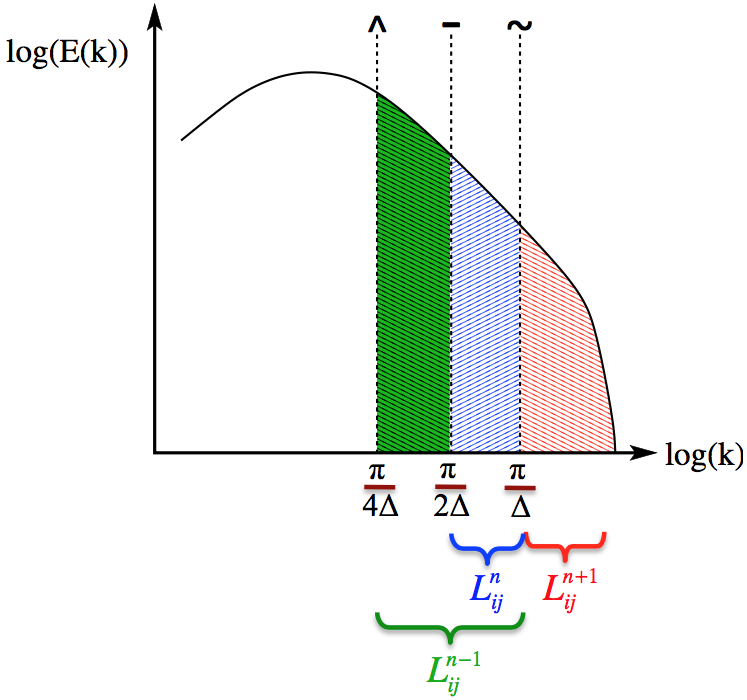
\includegraphics[width=0.65\textwidth]{scalesimilarity}	
\end{figure}
~\\Liu et al. (1994) found that the band between $\Delta$ ($\sim$) and $4\Delta$ (\textasciicircum) provided the best estimate. For $q_i$:
\begin{align*}
q_i^{n-1} &= \overline{(\widetilde{u}_i  - \hat u_i)(\widetilde{\theta} - \hat \theta)} - \overline{(\widetilde{u}_i  - \hat u_i)}\overline{(\widetilde{\theta} - \hat \theta)}\\
&= \overline{\widetilde u_i \widetilde \theta - \hat u_i \widetilde \theta - \widetilde u_i \hat \theta + \hat u_i \hat \theta} - \overline{(\widetilde{u}_i  - \hat u_i)}\overline{(\widetilde{\theta} - \hat \theta)}
\end{align*}
Assume (\textasciicircum) terms are constant under the (-) operator
\begin{align*}
q_i &= \overline{ \widetilde u_i \widetilde \theta} - \cancelto{}{\hat u_i \overline{\widetilde \theta}} - \cancelto{}{\overline{\widetilde u_i} \hat \theta} - \cancelto{}{\hat u_i \hat \theta} - \overline{\tilde u_i}\overline{\tilde \theta} + \cancelto{}{\hat u_i \overline{\widetilde \theta}} + \cancelto{}{\overline{\widetilde u_i} \hat \theta} + \cancelto{}{\hat u_i \hat \theta}\\
q_i &= \overline{ \widetilde u_i \widetilde \theta} - \overline{\tilde u_i}\overline{\tilde \theta}\\
q_i &= L_{i\theta}
\end{align*}
We assume that there is a similarity between $q_i$ and $L_{i\theta}$. We choose a linear relationship
$$\boxed{q_i = C_L L_{i\theta}}$$
where experimental data has shown $C_L\sim 1$.
}

\item Derive a scale-dependent dynamic model for the SFS stress based on the Wong-Lilly model (Wong, Lilly; Phys. Fluids, 1994) for the SFS
stress given by:
\begin{displaymath}
\tau_{ij}-\frac{1}{3}\tau_{kk}=-2C_{\epsilon}\Delta^{4/3}\widetilde{S}_{ij}
\end{displaymath}
You will need to use Germano's identity (Germano et al., Phys. Fluids, 1991) at two different scales to do this and you should end up with an algebraic expression for $C_{\epsilon}$, where $C_{\epsilon}$ is a function of $\Delta$ (and the resolved velocity field).  Clearly state all assumptions that you make along the way.\\
\textcolor{blue}{Using the Germano identity, $L_{ij} = T_{ij} - \overline{\tau}_{ij}$, where $L_{ij}$ is the Leonard stress and $T_{ij}$ is the SFS stress term applied at a test filter (denoted $-$) width $(\alpha \Delta$).\\\\
Let's look at the Germano identity for a filter width of $\Delta$ ($\sim$) and a test filter width of $2\Delta$ ($-$). We will assume that the Wong-Lilly model is applicable at our multiple filter widths. Scale-invariance is not assumed, so we introduce a scale-dependent term that follows a power-law distribution at the smallest resolved scales (\textit{i.e.}, $C_{\epsilon, 2\Delta}/C_{\epsilon} = C_{\epsilon, 4\Delta}/C_{\epsilon, 2\Delta}$), which is given by $\beta = C_{\epsilon, 2\Delta}/C_{\epsilon}$ and $\beta^2 = C_{\epsilon, 4\Delta}/C_{\epsilon}$:
\begin{align*}
T_{ij} (2\Delta) &= -2C_{\epsilon, 2\Delta} (2\Delta)^{4/3} \overline{\widetilde{S}}_{ij}\\
\bar \tau_{ij} &= -2C_{\epsilon} \Delta^{4/3} \overline{\widetilde{S}}_{ij}\\
L_{ij, 2\Delta} &= T_{ij} (2\Delta) - \bar \tau_{ij}\\
&= -2C_{\epsilon, 2\Delta} (2\Delta)^{4/3} \overline{\widetilde{S}}_{ij} + 2C_{\epsilon} \Delta^{4/3} \overline{\widetilde{S}}_{ij}\\
&= -2C_{\epsilon} 2^{4/3} \Delta^{4/3} \overline{\widetilde{S}}_{ij} \beta + 2C_{\epsilon} \Delta^{4/3} \overline{\widetilde{S}}_{ij}\\
\Aboxed{&=-2C_{\epsilon} \Delta^{4/3} \overline{\widetilde{S}}_{ij} (2^{4/3}\beta -1)}
\end{align*}
Similarly, when applied at a test filter width of $4\Delta$:
\begin{align*}
T_{ij} (4\Delta) &= -2C_{\epsilon, 4\Delta} (4\Delta)^{4/3} \overline{\widetilde{S}}_{ij}\\
\bar \tau_{ij} &= -2C_{\epsilon} \Delta^{4/3} \overline{\widetilde{S}}_{ij}\\
L_{ij, 2\Delta} &= T_{ij} (2\Delta) - \bar \tau_{ij}\\
&= -2C_{\epsilon, 4\Delta} (4\Delta)^{4/3} \overline{\widetilde{S}}_{ij} + 2C_{\epsilon} \Delta^{4/3} \overline{\widetilde{S}}_{ij}\\
&= -2C_{\epsilon} 4^{4/3} \Delta^{4/3} \overline{\widetilde{S}}_{ij} \beta^2 + 2C_{\epsilon} \Delta^{4/3} \overline{\widetilde{S}}_{ij}\\
\Aboxed{&=-2C_{\epsilon} \Delta^{4/3} \overline{\widetilde{S}}_{ij} (4^{4/3}\beta^2 -1)}
\end{align*}
~\\
Next, we define our error for the $2\Delta$ test filter, assume the Leonard stress is trace-free, and minimize the error using a least-squares approach:
$$e_{ij}^2 = (L_{ij} - C_{\epsilon}M_{ij})^2, \quad \text{where} \quad M_{ij} = -2\Delta^{4/3}\overline{\widetilde{S}}_{ij} (2^{4/3}\beta -1)$$
$$\frac{\partial e^2_{ij}}{\partial C_{\epsilon}} = -2L_{ij}M_{ij} + 2C_{\epsilon}M_{ij}M_{ij} = 0$$
$$C_{\epsilon} =\frac{\langle L_{ij} M_{ij} \rangle}{\langle M_{ij} M_{ij} \rangle}$$ 
We repeat the procedure for the $4\Delta$ test filter:
$$e_{ij}^2 = (L_{ij} - C_{\epsilon}N_{ij})^2, \quad \text{where} \quad N_{ij} = -2\Delta^{4/3}\overline{\widetilde{S}}_{ij} (4^{4/3}\beta^2 -1)$$
$$\frac{\partial e^2_{ij}}{\partial C_{\epsilon}} = -2L_{ij}N_{ij} + 2C_{\epsilon}N_{ij}N_{ij} = 0$$
$$C_{\epsilon} =\frac{\langle L_{ij} N_{ij} \rangle}{\langle N_{ij} N_{ij} \rangle}$$ 
Equating the two expressions for $C_\epsilon$ yields
$$\langle L_{ij} M_{ij} \rangle \langle N_{ij} N_{ij} \rangle - \langle L_{ij} N_{ij} \rangle \langle M_{ij} M_{ij} \rangle = 0$$
From this we can construct an algebraic expression for $\beta$ via $M_{ij}$ and $N_{ij}$. Once we have $\beta$, we can compute $M_{ij}$, and thus $C_\epsilon$.
}

\end{enumerate}

\end{document}